\documentclass{article}

\usepackage{tikz}
\usetikzlibrary{braids}

\begin{document}

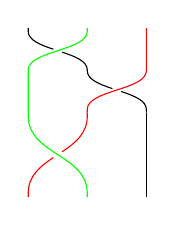
\begin{tikzpicture}
\pic[
  name prefix=mybraid 1,
  braid/.cd,
  number of strands=3,
  strand 1/.style={black},
  strand 2/.style={green},
  strand 3/.style={red},
  height=-.5cm,
  width=0.75cm,
  nudge factor=0.01,
  border height=1pt,
] {braid={s_1^{-1} s_2^{-1} }};
\pic[
  at={(mybraid 1-rev-1-e)},
  name prefix=mybraid 2,
  braid/.cd,
  number of strands=3,
  strand 3/.style={black},
  strand 1/.style={green},
  strand 2/.style={red},
  height=-1cm,
  width=0.75cm,
  nudge factor=0.01,
  border height=1pt,
] {braid={s_1 }};
\end{tikzpicture}
\end{document}
